\section{Galoistheorie}
\label{sec:galoistheorie}
\subsection{Galoisgruppen}
\label{subsec:galoisgruppen}
\begin{definition}{Galoisgruppe}{galoisgruppe}
Sei $f(x) \in \Q[x]$ ein Polynom mit rationalen Koeffizienten von Grad $\deg f = n \geq 1$ und seien $\lambda_1, \dots, \lambda_n \in \C$ die komplexen Nullstellen (mit Vielfachheiten) von $f(x)$. Die \textbf{Galoisgruppe}
\begin{equation}
\Gal(f) \leq \Sf_n
\end{equation} 
von $f$ über $\Q$ ist die Untergruppe der Permutationen $\sigma \in \Sf_n$, die die folgende Bedingung erfüllen:\\
Für jedes $r(x_1, \dots, x_n) \in \Q[x_1, \dots, x_n]$ mit $r(\lambda_1, \dots, \lambda_n) = 0$ gilt auch 
\begin{equation}
r(\lambda_{\sigma(1)}, \dots, \lambda_{\sigma(n)}) = 0.
\end{equation}
\end{definition}
Anders ausgedrückt ist $\Gal (f)$ also die Untergruppe derjenigen Permutationen, die alle algebraischen Relationen über $\Q$ der Nullstellen von $f(x)$ erhalten.
\begin{beispiel}
Betrache $f(x) = x^4-2 \in \Q[x]$ mit Nullstellen $a = \sqrt[4]{2}$, $b= i \sqrt[4]{2}$, $c=- \sqrt[4]{2}$ und $c=-i \sqrt[4]{2}$. Aus $x^4-2= (x-a)(x-b)(x-c)(x-d)$ folgen die Relationen:
\begin{equation}
\begin{split}
abcd &= -2\\
abc+abd+acd+bcd &= 0 \\
ab+ac+ad+bc+bd+cd &= 0\\
a+b+c+d &= 0.
\end{split}
\end{equation}
Zusätzlich gilt
\begin{equation}
\begin{split}
a^2b^2 &= -2\\
b^2c^2 &= -2\\
c^2d^2 &= -2\\
d^2a^2 &= -2.
\end{split}
\end{equation}
sowie
\begin{equation}
\begin{split}
a^2c^2 &= 2\\
b^2d^2 &= 2.
\end{split}
\end{equation}
Also definiert $\{a,b,c,d\}$ die Eckpunkte eines Quadrats:
\begin{center}
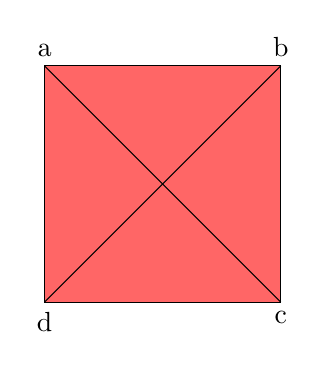
\begin{tikzpicture}
	\fill[fill=red!60!white, draw=black] (0,0) rectangle (3,3);
 	\draw (0,0) node[below] {d} -- (0,3);
 	\draw (0,3) node[above] {a} -- (3,3);
 	\draw (3,3) node[above] {b} -- (3,0);
 	\draw (3,0) node[below] {c} -- (0,0);
 	\draw (0,0) -- (3,3);
 	\draw (0,3) -- (3,0);
\end{tikzpicture}  
\end{center}
wobei die ersten vier Gleichungen die Kanten und die letzten zwei Gleichungen die Diagonalen repräsentieren. Die Relationen können also nur von Permutationen der Diedergruppe erhalten werden, sodass 
\begin{equation}
\Gal (f) \leq D_4 = \langle (1234), (12)(34) \rangle \leq \Sf_4
\end{equation}
gelten muss. Unklar ist (noch), ob tatsächlich $\Gal (f) = D_4$ gilt.
\end{beispiel}
\subsection{Körpererweiterungen}
\label{subsec:koerpererweiterungen}
\begin{definition}{Unterkörper und Körpererweiterung}{unterkoerper}
Sei $\L$ ein Körper. Ein \textbf{Unterkörper} $\K \sub \L$ ist eine Teilmenge, die beide neutralen Elemente von $(\L, +, \cdot)$ enthält und mit den auf $\K$ eingeschränkten Verknüpfungen wieder einen Körper bildet.\\
Anders herum nennen wir bei gegebenem $\K$ den Körper $\L$ \textbf{Körpererweiterung} von $\K$ und schreiben $\L \mid \K$.
\end{definition}
\begin{definition}{Grad der Körpererweiterung}{gradkoerpererweiterung}
Seien $\L$ und $\K$ Körper mit $\L \mid \K$. Dann können wir $\L$ als $\K$-Vektorraum auffassen und bezeichnen mit
\begin{equation}
[\L : \K] = \dim_\K \L
\end{equation}
den \textbf{Grad} von $\L \mid \K$. Darüber hinaus nennen wir $\L \mid \K$ \textbf{endlich}, falls $[\L : \K]$ endlich ist.
\end{definition}
\begin{lemma}{Faktorisierung des Grades}{faktorisierunggrad}
Seien $\M \mid \L$ und $\L \mid \K$ Körpererweiterungen. Dann ist $\M \mid \K$ genau dann endlich, wenn $\M \mid \L$ und $\L \mid \K$ endlich sind. Insbesondere gilt dann:
\begin{equation}
[\M : \K] = [\M : \L][\L : \K].
\end{equation}
\end{lemma}
\begin{beweis}
Betrachte Teilmengen $P:= \{m_1, \dots, m_r\} \sub \M$ und $Q:=\{l_1, \dots, l_s\} \sub \L$ sowie
\begin{equation}
QP:=\{l_im_j \mid 1 \leq i \leq s, 1 \leq j \leq r\}.
\end{equation}
Die Aussage folgt direkt aus den beiden Erkenntnissen:
\begin{enumerate}
\item Sei $P$ linear unabhängig über $\L$ und $Q$ über $\K$, dann ist $QP$ linear unabhängig über $\K$.
\item Sei $P$ erzeugend über $\L$ und $Q$ über $\K$, dann ist $QP$ erzeugend über $\K$.
\end{enumerate}
Diese Behauptungen folgen direkt aus der Umformung
\begin{equation}
\sum_{i,j} \lambda_{ij} l_im_j = \sum_j \left( \sum_i \lambda_{ij} l_i \right) m_j.
\end{equation}
\end{beweis}
\begin{beispiele}
\begin{enumerate}
\item $\C \mid \R$ ist eine Körpererweiterung von Grad $2$.
\item $\R \mid \Q$ ist eine Körpererweiterung unendlichen Grades. Betrachte dazu z.B. die linear unabhängige Teilmenge $\{1,\pi,\pi^2,\dots\} \sub \R$ über $\Q$.
\item Sei $\K$ ein Körper und $\K(x)=(\K[x] \exc \{0\})^{-1}\K[x]$ der zugehörige Quotientenkörper. Letzterer wird in diesem Fall als \textbf{Körper der rationalen Funktionen} bezeichnet. Dann ist $\K(x) \mid \K$ eine Körpererweiterung mit $[\K(x):\K] = \infty$. Betrachte dafür z.B. die über $\K$ linear unabhängige Teilmenge $\{1,x,x^2,\dots\}$.
\item Sei $f(x) \in \Q[x]$ ein Polynom von Grad $n \geq 1$ mit Nullstellen $\lambda_1, \dots, \lambda_n \in \C$. Sei $\Q(f)$ das Bild des Ringhomomorphismus
\begin{equation}
\begin{split}
\phi: \Q[x_1, \dots, x_n] &\to \C\\
f(x_1, \dots, x_n) &\mapsto f(\lambda_1, \dots, \lambda_n).
\end{split}
\end{equation}
Dann ist $\Q(f) \mid \Q$ eine endliche Körpererweiterung von Grad $\leq n^n$.
\end{enumerate}
\end{beispiele}
\begin{übung}
Zeige die Behauptung in Beispiel 4. Zeige insbesondere, dass $\Q(f)$ ein Körper ist.
\end{übung}

\subsection{Körperautomorphismen}
\label{subsec:koerperautomorphismen}
\begin{definition}{Körperautomorphismus}{koerperautomorphismus}
Sei $\L$ ein Körper. Ein bijektiver Ringhomomorphismus $\sigma: \L \to \L$ heißt \textbf{Körperautomorphismus} von $\L$. Die Menge der Körperautomorphismen von $\L$ wird mit $\Aut (\L)$ bezeichnet.
\end{definition}
\begin{definition}{Galoisgruppe der Körpererweiterung}{galoisgruppeerweitert}
Sei $\L \mid \K$ eine Körpererweiterung. Dann ist die \textbf{Galoisgruppe von $\L$ über $\K$} definiert als
\begin{equation}
\Gal (\L \mid \K) := \{\sigma \in \Aut(\L) \mid \forall x \in \K: \sigma(x) = x \}\leq \Aut(\L).
\end{equation}
\end{definition}
\begin{satz}{Kardinalität der Galoisgruppe ist beschränkt}{kardgalois}
Sei $\L \mid \K$ eine Körpererweiterung. Dann gilt
\begin{equation}
|\Gal (\L \mid \K)| \leq [\L : \K].
\end{equation}
\end{satz}
\begin{lemma}{Dedekind-Lemma}{dedekindlemma}
Seien $\L$ und $\E$ Körper, $\sigma_i: \L \to \E$ paarweise verschiedene Ringhomomorphismen mit $1 \leq i \leq n$ und $\lambda_i \in \E$ mit
\begin{equation} 
\sum_{i=1}^n \lambda_i \sigma_i =0 \in \text{Abb} (\L,\E).
\end{equation}
Diese Gleichung ist im $\E$-Vektorraum $\text{Abb}(\L,\E)$ aufzufassen. Dann gilt für alle $1 \leq i \leq n$, dass $\lambda_i =0$.
\end{lemma}
\begin{beweis}
Wir beweisen durch vollständige Induktion nach $n$. Für $n=1$ folgt die Behauptung aus $0 = \lambda_1 \sigma_1 = \lambda_1$. Sei nun $n>1$. Angenommen, es gäbe eine nichttriviale Linearkombination $\sum_{i=1}^n \lambda_i \sigma_i = 0$. O.B.d.A. sei $\lambda_1 \neq 0$. Wähle $a \in \L$ mit $\sigma_1(a)\neq \sigma_n(a)$. Dann gilt für alle $x \in \L$:
\begin{equation}
0 = \sum_{i=1}^n \lambda_i \sigma_i (ax) - \sigma_n(a) \sum_{i=1}^n \lambda_i \sigma_i (x) = \sum_{i=1}^{n-1} \lambda_i(\sigma_i(a)-\sigma_n(a))\sigma_i(x).
\end{equation} 
Dies ist aber eine kürzere Linearkombination der $\sigma_1, \dots, \sigma_{n-1}$ zu $0$, welche nicht-trivial ist, da $\lambda_1(\sigma_1(a)-\sigma_n(a))\neq 0$ nach Konstruktion. Dies ist ein Widerspruch.
\end{beweis}

\begin{satz}{Ringhomomorphismen beschränken Erweiterungsgrad}{homsbeschraenkenerweiterung}
Seien $\L \mid \K$ und $\E \mid \K$ Körpererweiterungen. seien weiterhin $\sigma_1, \sigma_2, \dots, \sigma_n$ paarweise verschiedene Ringhomomorphismen $\sigma_i: \L \to \E$ mit $\sigma_i|_{\K}=\id_\K$. Dann gilt:
\begin{equation}
n \leq [\L : \K].
\end{equation}
\end{satz}
\begin{beweis}
Falls $[\L : \K] = \infty$ gilt, ist die Aussage trivial. Sei also $[\L : \K] = m < \infty$ und sei $(e_1, e_2, \dots, e_m)$ eine $\K$-Basis von $\L$. Das LGS
\begin{equation}
\E^{m \times n} \ni \mat{\sigma_1(l_1), \cdots, \sigma_n(l_1)}{\sigma_1(l_2), \cdots, \sigma_n(l_2)}{\vdots, \vdots, \vdots}{\sigma_1(l_m), \cdots, \sigma_n(l_m)} \cvc{x_1, x_2, \vdots, x_n} = \cvc{0,0,\vdots,0}.
\end{equation}
Falls $n>m$ gilt, existiert eine nicht-triviale Lösung $(\lambda_1, \dots, \lambda_n) \in \E^n$, also 
\begin{equation}
\sum_{i=1}^n \lambda_i \sigma_i = 0.
\end{equation}
Dies ist ein Widerspruch zu Lemma \ref{dedekindlemma}.
\end{beweis}
\begin{korollar}{Aus Satz \ref{homsbeschraenkenerweiterung}}{aus335}
Satz \ref{kardgalois} folgt direkt.
\end{korollar}
\subsection{Galoiserweiterungen}
\label{subsec:galoiserweiterungen}

\begin{definition}{Galoiserweiterung}{galoiserweiterung}
Eine endliche Körpererweiterung $\L \mid \K$ heißt \textbf{Galoiserweiterung}, falls 
\begin{equation}
|\Gal (\L \mid \K)| = [\L : \K].
\end{equation}
\end{definition}
\begin{definition}{Fixkörper}{fixkörper}
Sei $\L$ ein Körper und $G \leq \Aut(\L)$. Der Unterkörper
\begin{equation}
\L^G := \{ x \in \L | \forall \sigma \in G: \sigma(x) = x\} \sub \L
\end{equation}
heißt \textbf{Fixkörper} von $G$.
\end{definition}
\begin{übung}
Zeige, dass $\L^G$ tatsächlich ein Unterkörper ist.
\end{übung}
\begin{satz}{Fixkörper ist Grundkörper}{fixkoepergrundkoerper}
Sei $\L \mid \K$ eine Galoiserweiterung mit $G = \Gal(\L \mid \K)$. Dann gilt $\L^G = \K$.
\end{satz}
\begin{beweis}
Direkt aus den Definitionen folgt, dass $\Gal(\L \mid \K) = \Gal(\L \mid \L^G)$. Weiterhin gilt $\K \sub \L^G \sub \L$. Da $\L \mid \K$ galoissch ist, gilt $|G|=[\L : \K]$. Aus Satz \ref{kardgalois} folgt, dass
\begin{equation}
[\L :\K] = |G| = |\Gal(\L \mid \L^G)| \leq [\L : \L^G]
\end{equation}
gilt, also
\begin{equation}
[\L:\L^G] = [\L : \K] \implies [\L^G : K] = 1 \implies \L^G = \K.
\end{equation}
\end{beweis}
\begin{übung}
Begründe, warum die letzte Implikation gelten muss.
\end{übung}
\begin{satz}{Satz von Artin}{artin}
Sei $\L$ ein Körper und $G \leq \Aut (\L)$. Dann gilt
\begin{equation}
[\L: \L^G] = |G|.
\end{equation}
Falls $G$ endlich ist, ist damit insbesondere die Körpererweiterung $\L \mid \L^G$ galoissch mit Galoisgruppe $G$.
\end{satz}
\begin{beweis}
Sei $\K := \L^G$. Wegen $G \leq \Gal(\L \mid \K)$ gilt
\begin{equation}
|G| \leq |\Gal(\L : \K)| \leq [\L : \K].
\end{equation}
Wir zeigen nun $[\L:\K] \leq |G|$. Ist $|G|=\infty$, ist die Aussage trivial, also sei $|G|=n<\infty$. Wir zeigen, dass je $n+1$ Elemente $x_1, x_2, \dots, x_{n+1} \in \L$ linear abhängig über $\K$ sind. Betrachte dazu für $G=\{\sigma_1, \sigma_2, \dots, \sigma_n\}$ das $\L$-lineare Gleichungssystem
\begin{equation}
\sum_{j=1}^{n+1} y_j \sigma_i(x_j) = 0
\end{equation}
für $1 \leq i \leq n$. Dieses LGS hat $n+1$ Variablen und $n$ Gleichungen, also existiert eine nicht-triviale Lösung $(\lambda_1, \lambda_2, \dots, \lambda_{n+1}) \in \L^{n+1}$. Sei o.B.d.A. $\lambda_1 \neq 0$. Für $1 \leq i \leq n$ wenden wir $\sigma_i^{-1}$ auf die $i$-te Gleichung an und erhalten
\begin{equation}
\sum_{j=1}^{n+1} \sigma_i^{-1}(\lambda_j) \cdot x_j = 0
\end{equation}
für $1 \leq i \leq n$. Summiere über alle Gleichungen:
\begin{equation}
\sum_{j=1}^{n+1} \underbrace{\alpha_j}_{\in \K} x_j = 0
\end{equation}
mit
\begin{equation}
\alpha_j = \sum_{i=1}^n \sigma_i^{-1}(\lambda_j)=\sum_{\sigma \in G} \sigma(\lambda_j) \in \L^G,
\end{equation}
da für die Gruppe $G$ Inversenbildung $g \mapsto g^{-1}$ eine Bijektion ist und die Summe invariant unter Wirkung von $G$ ist. Es bleibt noch, zu zeigen, dass die Koeffizienten $\alpha$ nicht-trivial sind. Wegen des Dedekind-Lemmae gilt $\sum_{\sigma \in G} \sigma \neq 0$, es gibt also $l \in \L$ mit $\sum_{\sigma \in G} \sigma (l)\neq 0$. Ersetze den Lösungsvektor $(\lambda_1, \lambda_2, \dots, \lambda_{n+1})$ durch die Reskalierung $l\cdot \lambda_1^{-1} \in \L$, also:
\begin{equation}
\left( (l\lambda_1^{-1}) \lambda_1, (l\lambda_1^{-1}) \lambda_2, \dots, (l\lambda_1^{-1}) \lambda_{n+1} \right) \in \L^{n+1}.
\end{equation}
Daraus folgt, dass
\begin{equation}
\alpha_1 = \sum_{\sigma \in G} \sigma(l) \neq 0 ,
\end{equation}
also liegt eine nicht-triviale $\K$-Linearkombination vor.
\end{beweis}
\begin{korollar}{Aus Satz \ref{artin}}{ausartin}
Sei $\L \mid \K$ eine endliche Körpererweiterung. Dann gilt:
\begin{equation}
|\Gal(\L \mid \K)| \mid [\L : \K]
\end{equation}
\end{korollar}
\begin{beweis}
Aus dem Satz von Artin folgt, dass
\begin{equation}
|\Gal(\L \mid \K)| = |\Gal(\L \mid \L^G)| = [\L : \L^G] \mid [\L : \K]
\end{equation}
\end{beweis}

\subsection{Galoiskorrespondenz}
\label{subsec:galoiskorrespondenz}

Sei $\L \mid \K$ eine Körpererweiterung mit Galoisgruppe $\Gal(\L\mid \K) =: G$. Betrachte die Mengen
\begin{equation}
\Uc(G) = \{H | H \leq G\}
\end{equation}
der Untergruppen von $G$ und
\begin{equation}
\Zc(\L \mid \K) := \{\M | \K \sub \M \sub \L\}.
\end{equation}
der Zwischenkörper von $\K$ und $\L$. Die Körper $\K$ und $\M$ heißen Unterkörper, $\M$ heißt Zwischenkörper von $\K$ und $\L$.
\begin{theorem}{Galoiskorrespondenz}{galoiskorrespondenz}
Sei $\L \mid \K$ eine Galoiserweiterung mit Galoisgruppe $Gal(\L \mid \K)$. Dann sind die Abbildungen
\begin{equation}
\begin{split}
\Uc (G) &\to \Zc (\L \mid \K)\\
H &\mapsto L^H
\end{split}
\end{equation}
und
\begin{equation}
\begin{split}
\Zc (\L \mid \K) &\to \Uc (G)\\
M &\mapsto \Gal(\L \mid \M)
\end{split}
\end{equation}
zueinander inverse Bijektionen.
\end{theorem}
\begin{beispiel}
Sei $\L \mid \K$ eine Galoiserweiterung mit $\Gal(\L \mid \K) \cong \Sf_3$. Diese Gruppe verstehen wir bereits: (Diagramm einfügen)
\end{beispiel}
\begin{beweis}
$g \circ f = \id$ ist klar, da
\begin{equation}
H = \Gal(\L \mid \L^H)
\end{equation}
nach dem Satz von Artin.
\end{beweis}
